
\chapter{Feedforward Neural Network Models}

In this chapter, we describe two feedforward network models: Feedforward-History and Feedforward-CRF. Then, we show the performance and decoding speed of different feedforward models on POS and NER. 

\section{Network Architecture}

\subsection{Feedforward-History Model}

Inspired by the greedy parser system by ~\cite{chen2014fast}, we present a similar greedy transition system for sequence tagging in this section. The greedy parser system employs a basic arc-standard system (~\citeauthor{nivre2004deterministic}, ~\citeyear{nivre2004deterministic}), which consists of three types of transitions(LEFT-ARC, RIGHT-ARC, and SHIFT), a stack, and a buffer. While the greedy parser system has three types of actions, the sequence tagging system only needs SHIFT action which predicts the tag of the current word in the buffer and shifts the word to the stack. 

In this greedy tagging system, we use a feedforward network to make decisions on individual words, and assume that the word to be labeled depends mainly on its neighbor words instead of the whole sentence. Besides the word features, the system also takes into account the lexical composition of the words (spelling features), and the previous tagging decisions (history features). Thereby, we represent this architecture as the Feedforward-History model. The way Feedforward-History incorporates word features is the same with the window approach proposed in ~\cite{collobert2011natural}. The difference between these two models is that Feedforward-History uses spelling features and history features while the model of ~\cite{collobert2011natural} only uses word features.

\begin{figure}
  \centering
  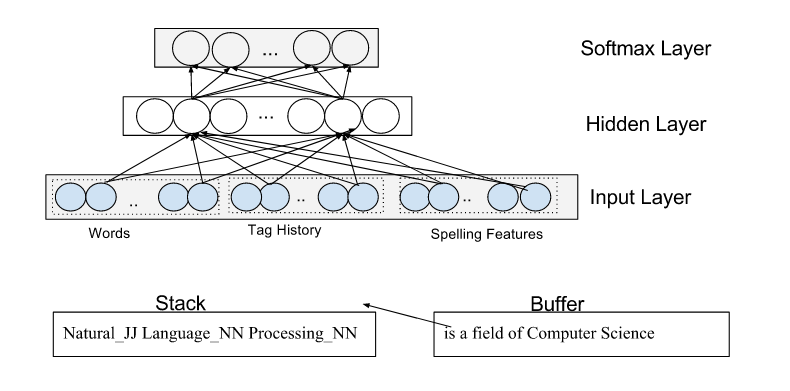
\includegraphics[scale=0.6]{greedypos.png}
 \caption{The architecture of the greedy tagging system using the Feedforward-History model.}
  \label{fig:greedypos}
\end{figure}

Figure \ref{fig:greedypos} illustrates the process of how the greedy tagging system uses Feedforward-History to decode a POS example. Since the current word only depends on its neighbors in this greedy tagging system, we use a fixed size window around the current word to generate features. In order to generate features for the words at the beginning and at the end of the sentence, we add special padding word at the beginning and at the end. To generate dense word features, we convert each word in the input sequence to a $d$-dimensional vector representation $e_{w_{i}}$. Meanwhile, we have a full vocabulary embedding vector dictionary $E_{w}$. Given a word $w_{i}$, we look up its embedding vector $e_{w_{i}}$ in $E_{w}$. According to \cite{ratnaparkhi1996maximum}, spelling features of a word can help predict the part-of-speech tag as well, such as upper and lower case features, prefix and suffix features. Each spelling feature of a word is also associate with an embedding vector $e_{s_{i}}$, and it can be looked up from a embedding vector dictionary $E_{s}$. Besides word features and spelling features, we incorporate the history label features in this model. Since the greedy sequence tagging system makes decision word by word in a sequence, we can only use the previous tags as input history features for predicting the current tag. Each history feature is represented as $e_{ht_{i}}$ and can be looked up from a label dictionary is $E_{HT}$.

The input layer $X=\left( x_{1},x_{2},\ldots x_{n}\right)$ to the feedforward network is obtained by concatenating the word feature vectors, spelling feature vectors, and history feature vectors. In general, generating a lot of hand-engineered features for sequence tagging are expensive: selecting useful features is an empirical process based on trials and errors, and computing features vectors requires searching feature strings in huge dictionaries and concatenating them together. We try to use features as little as possible to cut the time of feature generation while keeping the model accurate. In the implementation, we extract the word and spelling features on a window size of 8 centered on the current focused word. We extract the following spelling features of each word: whether it starts with a capital letter; whether it has all capital letters; whether it has a mix of letters and digits; whether if has punctuation; letter prefixes and suffices of length two and three. We also extract the history features from the previous four predicted tags. 

The input layer is the concatenation of the feature vectors of the focus word, and the the output layer is a probability distribution over tags. In order to build a simple and fast network model, we only use one hidden layer in this model. The input unit $x_{i}$ is mapped to a hidden unit $h_{i}$ through the rectifier activation function (ReLU):

\begin{equation}
ReLU\left(x\right) = \ln\left[1+\exp\left(x\right)\right]
\end{equation}

\begin{equation}
h_{i}=ReLU\left( W_{1}^{w}x_{i}^{w}+W_{1}^{s}x_{i}^{s}+W_{1}^{l}x_{i}^{l}+b_{1}\right),
\end{equation}

where $x^{w}$ represents the word input features, $x^{s}$ represents the spelling input features, $x^{l}$ represents history input features, $W_{1}$ is the weight parameters for the hidden layer, and $b_{1}$ is the bias of in the hidden layer. The output of the network is a probability distribution over tags, and its dimension is the size of the possible tags. Label probability distribution is modeled by a softmax layer:

\begin{equation}
p_{i}=softmax\left(W_{2}h_{i}+b_{2}\right),
\end{equation}

where $W_{2}$ is the weight parameter in the softmax layer and $b_{2}$ is the bias in the softmax layer.

The network is trained by minimizing a negative log likelihood over the training data. The embedding vectors are trained together with the weight vectors and bias in the network. We denote all trainable parameters as $\theta$. Given a sequence predictions, $Y=\left( y_{1},y_{2},\ldots y_{n}\right)$,
the score of the output sequence is the sum of the probability of each decision $y_{i}$: 

\begin{equation}
S\left( Y\right) = \sum _{i}^{n}p_{i}\left(y_{i}\right),
\end{equation}

and the loss function is:

\begin{equation}
L\left(\theta\right) = -log\left(\sum _{i}^{n}p_{i}\left(y_{i}\right)\right),
\end{equation}


\subsection{Feedforward-CRF}
\label{Feedforward-CRF}
There are two ways to make use of the output tag information: the first one is to use the previous predicted tags as input features to be fed into the feedforward network layer, as in Feedforward-History; the second one is to use CRF on sentence level output tags instead of individual tags as in the following model. Feedforward-CRF shares the same architecture with Feedforward-History except using CRF to model the output sequence after computing tag probability distribution for each individual word. Feedforward-History can perform well on some sequence tagging tasks in which output labels do not have strong correlations, such as POS. Some tasks have grammar constrains on the output tags so that the tags depend on their neighbors, such as NER. While Feedforward-History fails to take into account the grammar constrains on output tag sequence, Feedforward-CRF can make final decisions on the sentence level. Since the first part of the architecture is the same with Feedforward-History, we skip this part. We describe how to apply CRF to model the sequence in detail here.

Given a sequence of output predictions $y=\left( y_{1},y_{2},\ldots y_{n}\right)$,
The score of the output sequence is:

\begin{equation}
S\left( y\right)=\sum _{i}^{n}T_{i,i+1}+\sum _{i}^{n}p_{i}\left(y_{i}\right)
\end{equation}

where $T$ is a matrix of transition scores such that $T_{i,j}$ represents the score of a transition from the label $i$ to label $j$, $p_{i}\left(y_{i}\right)$ is the probability of $y_{i}$ being the label of word $i$.

During training, we score every possible output sequences, and use a softmax layer to generate the probability distribution of output sequences, shown in Equation \ref{eqn:softmax}. Then, we minimize the negative log likelihood over the training sentences. During decoding, we can recover the tag sequences of the test data using dynamic programming.

\begin{equation}\label{eqn:softmax}
P\left( y\right) = softmax(S\left( y\right))
\end{equation}


\section{Experiments and Results}
To evaluate the greedy tagging systems with feedforward models, we run our models (\ffa, \ffb) on POS and NER. We also compare their performance and decoding speed. The performance of POS is measured by the per word accuracy, and the performance of NER is measured by the F1 score. The speed is measured by the average number of sentences and words decoded per second. We also want to show the robustness of feedforward network models, so we build a model using a feedforward network with only word features, which serves as a baseline model in the experiments. We denote this baseline model as Feedforward in this thesis.

In the POS experiments, we train the models using the Penn Treebank training data and development data. Then, we decode the Penn Treebank test data with trained models and record the per word accuracy and decoding time. In the NER experiments, we train the models using the CoNLL 2003 training data and development data. Then we decode the test data with the trained models, and record the F1 score and decoding time. The details of the data set are shown in Table \ref{table:my-dataset}.

 
We implement the models using Python and the Tensorflow 1.0 library. We use the Glove pretrained word embedding where each word corresponds to a 100-dimensional embedding vector in NER experiments because of the lack of training data. We tune the hyper-parameters for training. Specifically we use Adam (~\citeauthor{kingma2014adam}, ~\citeyear{kingma2014adam}) for stochastic optimization, set the learning rate to be 0.001, and the hidden layer to be 128. We have the batch implementation which processes multiple sentences at the same time, and we set the batch size to be 32 in the experiments. We run all the experiments in this thesis on a GeForce GTX 1080 GPU. 

Table \ref{table:ff-table1} and Table \ref{table:ff-tabel2} demonstrate our final benchmark results of three feedforward models on POS and NER. Figure \ref{fig:ff} illustrates the performance of the three models in a bar chart. In POS, Feedforward is 1.39\% less accurate then \ffa. In NER, the F1 score of Feedforward is 2.42 lower than \ffa. Since only using word features does not decrease the POS performance dramatically, we can conclude that our greedy tagging systems with feedforward models do not heavily rely on spelling features. The spelling features are more helpful in NER then in POS. In both POS and NER, Feedforward-CRF has better performance than Feedforward-history, but it improves the performance more on NER because of the dependencies between the output tags in NER. Feedforward-CRF is slower than the Feedforward-History since the CRF model computes the score of every possible output sequences.

\begin{table}[]
\centering
\caption{Feedforward Models Accuracy and F1 Score}
\label{table:ff-table1}
\begin{tabular}{|c|c|c|}
\hline
Model         & POS (Accuracy)  & NER (F1 Score)       \\ \hline
Feedforward    & 95.89          &   84.12     \\ \hline
Feedforward-History & 97.28     & 86.54        \\ \hline
Feedforward-CRF     & 97.30          &   87.85     \\ \hline
\end{tabular}
\end{table}

\begin{table}[]
\centering
\caption{Feedforward Models Decoding Speed}
\label{table:ff-tabel2}
\begin{tabular}{|c|c|c|}
\hline
Model       & POS  (sentences, words/sec)  & NER  (sentences, words/sec)      \\ \hline
Feedforward    & 1319(30967)     & 2117(26819)    \\ \hline
Feedforward-History & 829(19474)     & 1390(17609)     \\ \hline
Feedforward-CRF    & 761(17877)     & 1374(17412)     \\ \hline
\end{tabular}
\end{table}

\begin{figure}
  \centering
  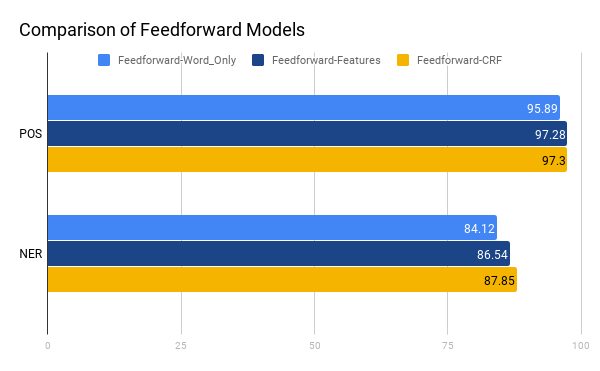
\includegraphics[scale=0.6]{ffbar.png}
 \caption{Performance comparison between Feedforward Models on POS and NER}
  \label{fig:ff}
\end{figure}
